\documentclass[12pt,a4paper]{article}
\usepackage[utf8]{vietnam}
\usepackage{amsmath,amssymb,amsfonts,mathrsfs}
\usepackage[left=1.5cm,right=1.5cm,top=2cm,bottom=2cm,headheight=18pt]{geometry}
\usepackage{enumitem}
\usepackage{array}
\usepackage{graphicx}
\usepackage{fancyhdr}

\pagestyle{fancy}
\fancyhf{}
\lhead{\small\textbf{HƯỚNG TỚI THPTQG 2027}}
\rhead{\small\textit{Người biên soạn: Dương Gia Bảo}}
\rfoot{\small Trang \thepage}
\renewcommand{\headrulewidth}{0.4pt}

\begin{document}

\noindent
\begin{minipage}[t]{0.40\textwidth}
    \centering
    \textbf{HƯỚNG TỚI THPTQG 2027}\\[-2pt]
    \rule{3.2cm}{0.6pt}\\[4pt]
    \textbf{ĐỀ CHÍNH THỨC}
\end{minipage}\hfill
\begin{minipage}[t]{0.58\textwidth}
    \centering
    \textbf{ĐỀ THI KHẢO SÁT CHẤT LƯỢNG}\\
    \textbf{ĐỀ SỐ 2}\\
    \textbf{Môn thi: TOÁN}\\
    \textit{\small Thời gian làm bài: 90 phút, không kể thời gian phát đề}
\end{minipage}

\vspace{0.2cm}
\noindent
\begin{minipage}[b]{0.78\textwidth}
    \textbf{Họ và tên:}\dotfill\textbf{SBD:}\makebox[3.5cm]{\dotfill}
\end{minipage}\hfill
\begin{minipage}[b]{0.20\textwidth}
    \hfill
    \setlength{\fboxrule}{0.8pt}%
    \fbox{\begin{minipage}{2.3cm}
        \centering
        \textbf{\small Mã đề thi}\\
        \textbf{0002}
    \end{minipage}}
\end{minipage}
\vspace{0.2cm}

% ==========================================
% PHẦN I
% ==========================================
\section*{\large PHẦN I. CÂU TRẮC NGHIỆM NHIỀU PHƯƠNG ÁN LỰA CHỌN}
\textit{Thí sinh trả lời từ câu 1 đến câu 12. Mỗi câu hỏi thí sinh chỉ chọn một phương án. Mỗi câu trả lời đúng được 0,25 điểm.}

\begin{enumerate}[label=\textbf{Câu \arabic*:}, leftmargin=*]

\item
\begin{minipage}[t]{\linewidth} 
Sau khi tiêm một liều thuốc kháng sinh cho bệnh nhân, nồng độ thuốc trong máu (đơn vị: mg/L) sau $t$ giờ ($t \ge 0$) được mô hình hóa bởi hàm số:
$$C(t) = \dfrac{40t}{t^2 + 4}$$
Hỏi sau bao nhiêu giờ kể từ thời điểm tiêm thuốc thì nồng độ thuốc trong máu bệnh nhân đạt mức cao nhất?
\begin{enumerate}[label=\Alph*., itemsep=0pt, topsep=3pt, parsep=0pt]
    \item $t = 2$ giờ.
    \item $t = 4$ giờ.
    \item $t = 1$ giờ.
    \item $t = 3$ giờ.
\end{enumerate}
\end{minipage}

\item
\begin{minipage}[t]{\linewidth} 
Mức cường độ âm $L$ (đơn vị: dB) được xác định bởi công thức $L = 10 \log_{10}\left(\dfrac{I}{I_0}\right)$, trong đó $I_0 = 10^{-12}\text{ W/m}^2$ là cường độ âm chuẩn và $I$ là cường độ âm tại điểm khảo sát. Tại một công trường xây dựng, một máy đóng cọc phát sóng âm lan truyền đẳng hướng trong không gian. Biết tại điểm $A$ cách máy $10\text{ m}$ có mức cường độ âm đo được là $90\text{ dB}$. Hỏi tại điểm $B$ cách máy $100\text{ m}$ thì mức cường độ âm đo được bằng bao nhiêu? (Bỏ qua sự hấp thụ âm của không khí).
\begin{enumerate}[label=\Alph*., itemsep=0pt, topsep=3pt, parsep=0pt]
    \item $80\text{ dB}$.
    \item $70\text{ dB}$.
    \item $60\text{ dB}$.
    \item $50\text{ dB}$.
\end{enumerate}
\end{minipage}

\item
\begin{minipage}[t]{\linewidth} 
Để kéo dãn một lò xo công nghiệp thêm một đoạn $x$ (mét) so với chiều dài tự nhiên, cần tác dụng một lực biến thiên theo hàm số $F(x) = 200x + 60x^2\text{ (N)}$. Công cơ học $W = \int_{x_1}^{x_2} F(x) dx$ cần thực hiện để kéo lò xo dãn từ $x = 0{,}1\text{ m}$ đến $x = 0{,}3\text{ m}$ bằng
\begin{enumerate}[label=\Alph*., itemsep=0pt, topsep=3pt, parsep=0pt]
    \item $9{,}20\text{ J}$.
    \item $7{,}84\text{ J}$.
    \item $8{,}52\text{ J}$.
    \item $10{,}56\text{ J}$.
\end{enumerate}
\end{minipage}

\item
\begin{minipage}[t]{\linewidth} 
Trong không gian $Oxyz$, một sườn đồi phẳng được mô hình hóa bởi mặt phẳng $(\alpha): 2x - 2y + z + 8 = 0$. Một trạm phát sóng viễn thông mặt đất đặt tại vị trí $A(1; 2; 3)$. Để trạm thu sóng $M$ trên sườn đồi nhận được tín hiệu mạnh nhất thì khoảng cách $AM$ phải ngắn nhất (tức $M$ là hình chiếu vuông góc của $A$ lên mặt phẳng $(\alpha)$). Tọa độ của trạm thu $M$ là
\begin{enumerate}[label=\Alph*., itemsep=0pt, topsep=3pt, parsep=0pt]
    \item $M(-1; 4; 2)$.
    \item $M(0; 2; -4)$.
    \item $M(1; -2; 1)$.
    \item $M(-3; 6; 1)$.
\end{enumerate}
\end{minipage}

\item
\begin{minipage}[t]{\linewidth} 
Một bệnh nhân điều trị bệnh mãn tính được chỉ định uống một liều thuốc $100\text{ mg}$ vào cùng một thời điểm mỗi ngày. Sau mỗi chu kỳ 24 giờ, cơ thể đào thải $60\%$ lượng thuốc hiện có và giữ lại $40\%$. Gọi $u_n$ là lượng thuốc (mg) có trong cơ thể bệnh nhân ngay sau khi uống liều thứ $n$. Sau thời gian dài điều trị liên tục ($n \to +\infty$), lượng thuốc tối đa tích lũy trong cơ thể bệnh nhân tiến tới giá trị nào sau đây?
\begin{enumerate}[label=\Alph*., itemsep=0pt, topsep=3pt, parsep=0pt]
    \item $250\text{ mg}$.
    \item $166{,}67\text{ mg}$.
    \item $150\text{ mg}$.
    \item $200\text{ mg}$.
\end{enumerate}
\end{minipage}

\item
\begin{minipage}[t]{\linewidth} 
Khảo sát đường kính (mm) của 50 chi tiết máy do một dây chuyền gia công tự động sản xuất thu được mẫu số liệu ghép nhóm sau:
\begin{center}
\begin{tabular}{|c|c|c|c|c|}
\hline
\textbf{Đường kính (mm)} & $[18; 20)$ & $[20; 22)$ & $[22; 24)$ & $[24; 26)$ \\ \hline
\textbf{Số chi tiết} & $10$ & $25$ & $10$ & $5$ \\ \hline
\end{tabular}
\end{center}
Độ lệch chuẩn $s$ của mẫu số liệu ghép nhóm trên bằng bao nhiêu (làm tròn kết quả đến hai chữ số thập phân)?
\begin{enumerate}[label=\Alph*., itemsep=0pt, topsep=3pt, parsep=0pt]
    \item $2{,}14\text{ mm}$.
    \item $3{,}04\text{ mm}$.
    \item $1{,}48\text{ mm}$.
    \item $1{,}74\text{ mm}$.
\end{enumerate}
\end{minipage}

\item
\begin{minipage}[t]{\linewidth} 
Một dây chuyền sản xuất vi mạch bán dẫn hoạt động ổn định với tỉ lệ sản phẩm lỗi là $2\%$. Lấy ngẫu nhiên một lô gồm 10 con chip để kiểm tra độc lập. Xác suất để trong lô kiểm tra có ít nhất một con chip bị lỗi xấp xỉ bằng
\begin{enumerate}[label=\Alph*., itemsep=0pt, topsep=3pt, parsep=0pt]
    \item $18{,}29\%$.
    \item $20{,}00\%$.
    \item $2{,}00\%$.
    \item $16{,}67\%$.
\end{enumerate}
\end{minipage}

\item
\begin{minipage}[t]{\linewidth} 
Một xét nghiệm sàng lọc bệnh truyền nhiễm có độ nhạy $96\%$ (xác suất người có bệnh nhận kết quả dương tính) và độ đặc hiệu $95\%$ (xác suất người không có bệnh nhận kết quả âm tính). Biết tỉ lệ mắc bệnh trong cộng đồng là $1\%$. Một người đi xét nghiệm ngẫu nhiên nhận kết quả dương tính. Xác suất người đó thực sự mắc bệnh xấp xỉ bằng
\begin{enumerate}[label=\Alph*., itemsep=0pt, topsep=3pt, parsep=0pt]
    \item $96{,}00\%$.
    \item $50{,}00\%$.
    \item $32{,}48\%$.
    \item $16{,}24\%$.
\end{enumerate}
\end{minipage}

\item
\begin{minipage}[t]{\linewidth} 
Cho hàm số $y = \dfrac{x^2 - 3x + 3}{x - 1}$. Khoảng cách giữa hai điểm cực trị của đồ thị hàm số bằng
\begin{enumerate}[label=\Alph*., itemsep=0pt, topsep=3pt, parsep=0pt]
    \item $4$.
    \item $2\sqrt{5}$.
    \item $2\sqrt{2}$.
    \item $5$.
\end{enumerate}
\end{minipage}

\item
\begin{minipage}[t]{\linewidth} 
Một trang trại điện mặt trời có công suất phát điện phụ thuộc thời gian trong ngày theo hàm số $P(t) = -t^3 + 9t^2 + 48t\text{ (kW)}$ với $t$ là số giờ tính từ 6 giờ sáng ($0 \le t \le 10$). Công suất phát điện lớn nhất của trang trại đạt được vào thời điểm nào trong ngày?
\begin{enumerate}[label=\Alph*., itemsep=0pt, topsep=3pt, parsep=0pt]
    \item $12$ giờ.
    \item $15$ giờ.
    \item $14$ giờ.
    \item $13$ giờ.
\end{enumerate}
\end{minipage}

\item
\begin{minipage}[t]{\linewidth} 
Một máy bay thương mại bay thẳng trên đoạn $AB$ từ $A(2; 1; 10)$ đến $B(8; 9; 10)$ (đơn vị: km, cao độ bay $10\text{ km}$). Một trạm quan sát ra-đa mặt đất đặt tại gốc tọa độ $O(0; 0; 0)$. Khoảng cách ngắn nhất từ trạm ra-đa đến các vị trí của máy bay trên đoạn $AB$ bằng
\begin{enumerate}[label=\Alph*., itemsep=0pt, topsep=3pt, parsep=0pt]
    \item $\sqrt{101}\text{ km}$.
    \item $10\text{ km}$.
    \item $\sqrt{105}\text{ km}$.
    \item $12\text{ km}$.
\end{enumerate}
\end{minipage}

\item
\begin{minipage}[t]{\linewidth} 
Một phôi gốm đặc dùng để chế tác bình hoa có dạng khối tròn xoay thu được khi quay hình phẳng giới hạn bởi đường cong $y = \sqrt{x} e^{x/2}$, trục hoành $Ox$ và hai đường thẳng $x = 0, x = 2$ xung quanh trục hoành $Ox$ (đơn vị trên các trục tọa độ là decimet). Thể tích phôi gốm đặc bằng
\begin{enumerate}[label=\Alph*., itemsep=0pt, topsep=3pt, parsep=0pt]
    \item $V = \pi(e^2 - 1)\text{ dm}^3$.
    \item $V = 2\pi e^2\text{ dm}^3$.
    \item $V = \pi(e^2 + 2)\text{ dm}^3$.
    \item $V = \pi(e^2 + 1)\text{ dm}^3$.
\end{enumerate}
\end{minipage}

\end{enumerate}

% ==========================================
% PHẦN II
% ==========================================
\newpage
\section*{PHẦN II. CÂU TRẮC NGHIỆM ĐÚNG/SAI}
\textit{Thí sinh trả lời từ câu 1 đến câu 4. Trong mỗi ý a), b), c), d) ở mỗi câu, thí sinh chọn Đúng hoặc Sai.}

\begin{enumerate}[label=\textbf{Câu \arabic*:}, leftmargin=*]

\item
\begin{minipage}[t]{\linewidth} 
Một tập đoàn công nghệ sản xuất thiết bị điện tử thông minh. Tổng chi phí sản xuất $x$ ngàn thiết bị ($0 < x < 25$) mỗi tháng là $C(x) = 2x^3 - 12x^2 + 30x + 40$ (triệu đồng). Giá bán mỗi ngàn thiết bị phụ thuộc vào lượng cung ứng theo hàm giá $p(x) = 150 - 6x$ (triệu đồng/ngàn thiết bị). Chính phủ áp mức thuế $t = 18$ triệu đồng trên mỗi ngàn thiết bị bán ra. Doanh thu của tập đoàn là $R(x) = x \cdot p(x)$ và lợi nhuận ròng sau thuế là $L(x) = R(x) - C(x) - 18x$.
\begin{enumerate}[label=\alph*)]
\item Hàm doanh thu bán $x$ ngàn thiết bị là $R(x) = 150x - 6x^2$ (triệu đồng).
\item Tại mức sản lượng $x = 3$ ngàn thiết bị, chi phí cận biên của tập đoàn là $MC(3) = C'(3) = 12$ triệu đồng/ngàn thiết bị.
\item Nếu chính phủ bãi bỏ thuế hoàn toàn ($t = 0$), mức lợi nhuận ròng tối đa của tập đoàn ở sản lượng nguyên $x = 5$ ngàn thiết bị sẽ tăng thêm $120$ triệu đồng so với khi có thuế.
\item Để đạt lợi nhuận ròng lớn nhất với số lượng nguyên ngàn thiết bị, tập đoàn nên sản xuất $5$ ngàn thiết bị mỗi tháng và lợi nhuận ròng tối đa đạt $370$ triệu đồng.
\end{enumerate}
\end{minipage}

\item
\begin{minipage}[t]{\linewidth} 
Một tên lửa thử nghiệm khí quyển được phóng thẳng đứng từ mặt đất. Kể từ thời điểm phóng $t = 0$ (giây), tên lửa có vận tốc ban đầu $v(0)=0$ và gia tốc tổng hợp (đã tính trọng lực) biến thiên theo thời gian $a(t) = 12t - 3t^2\text{ (m/s}^2\text{)}$ cho đến khi hết nhiên liệu tại $t = 4$ giây. Bỏ qua lực cản không khí. Sau $t = 4$ giây, tên lửa chuyển động tự do dưới tác dụng của trọng lực với gia tốc trọng trường $g = 10\text{ m/s}^2$.
\begin{center}
    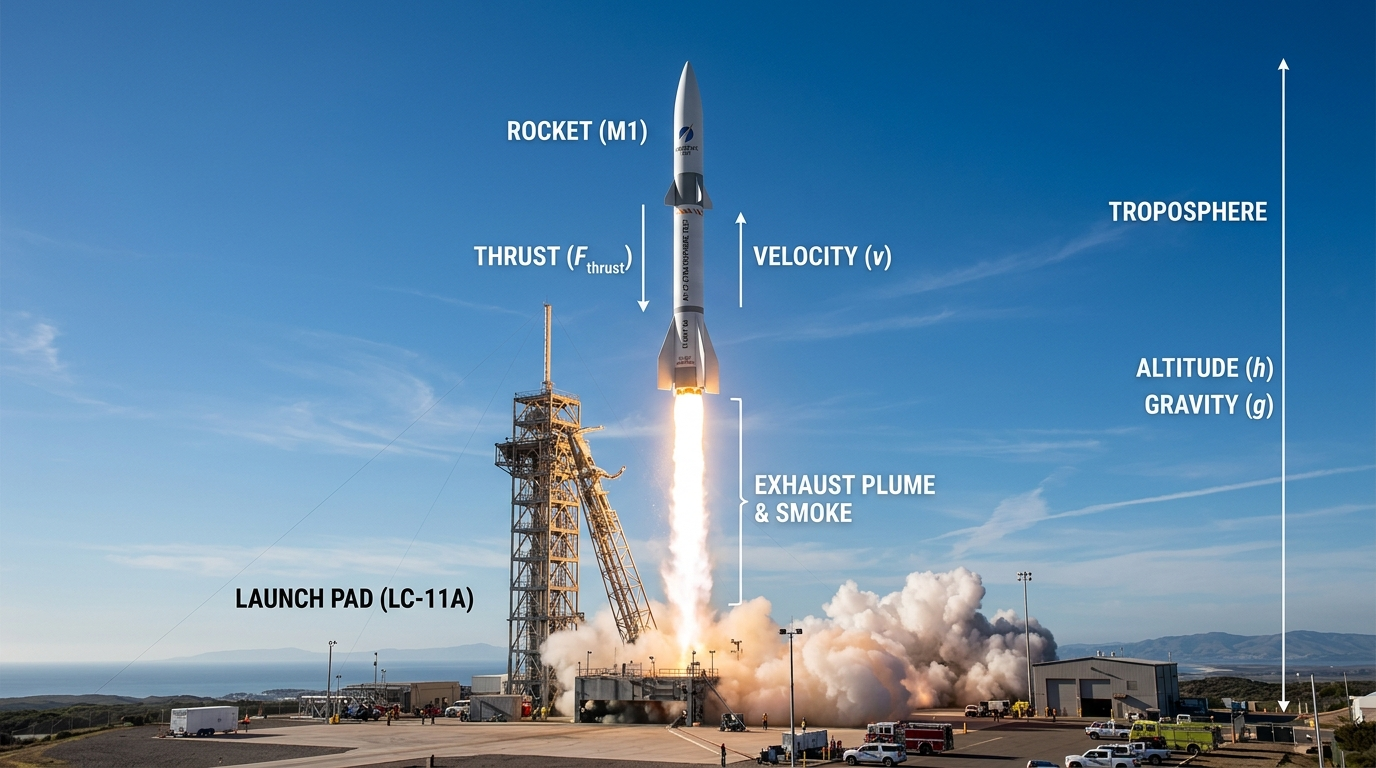
\includegraphics[width=0.48\textwidth]{images/phan2_cau2_tenlua.jpg}\\[2pt]{\footnotesize\itshape Hình minh họa bối cảnh; sử dụng số liệu trong đề.}
\end{center}
\begin{enumerate}[label=\alph*)]
\item Vận tốc của tên lửa tại thời điểm hết nhiên liệu $t = 4$ giây bằng $32\text{ m/s}$.
\item Tổng độ cao tối đa (so với mặt đất) mà tên lửa đạt được trong toàn bộ hành trình bằng $83{,}2\text{ m}$.
\item Độ cao của tên lửa đạt được tại thời điểm hết nhiên liệu $t = 4$ giây bằng $64\text{ m}$.
\item Kể từ thời điểm hết nhiên liệu $t = 4$ giây, tên lửa tiếp tục bay lên cao thêm trong $3{,}2$ giây nữa trước khi đạt đỉnh độ cao tuyệt đối.
\end{enumerate}
\end{minipage}

\item
\begin{minipage}[t]{\linewidth} 
Một công ty viễn thông triển khai hệ thống lọc tin nhắn rác tự động bằng trí tuệ nhân tạo (AI). Thực tế có $8\%$ tổng số tin nhắn gửi qua mạng là tin nhắn rác. Hệ thống AI có độ nhạy $95\%$ (nhận diện đúng $95\%$ tin nhắn rác) và tỉ lệ báo sai $4\%$ (báo nhầm $4\%$ tin nhắn hợp lệ là rác). Để tăng độ chính xác, tất cả các tin nhắn bị AI đánh dấu rác sẽ được chuyển qua Lớp kiểm định 2 do chuyên viên kiểm tra. Trong số tin nhắn rác được AI chuyển đến, chuyên viên phát hiện và chặn đúng $98\%$, bỏ sót $2\%$. Đối với tin nhắn hợp lệ được AI chuyển đến, chuyên viên không bao giờ nhận định nhầm thành rác. Tin nhắn chỉ bị chặn nếu cả hai lớp đều xác định là rác.
Chọn ngẫu nhiên một tin nhắn trong hệ thống mạng. Gọi $A$ là biến cố "Tin nhắn đó là tin nhắn rác" và $B$ là biến cố "Tin nhắn đó bị hệ thống AI đánh dấu là rác".
\begin{enumerate}[label=\alph*)]
\item Tỉ lệ tin nhắn hợp lệ bị hệ thống chặn nhầm hoàn toàn sau cả 2 lớp kiểm định bằng $3{,}68\%$.
\item Xác suất một tin nhắn ngẫu nhiên bị hệ thống AI đánh dấu là rác bằng $P(B) = 0{,}1128$.
\item Nếu một tin nhắn bị hệ thống AI đánh dấu là rác, xác suất tin nhắn đó thực sự là tin nhắn rác xấp xỉ $67{,}38\%$.
\item Xác suất một tin nhắn chọn ngẫu nhiên vừa là tin nhắn rác vừa bị cả hai lớp phát hiện và chặn lại bằng $0{,}07448$.
\end{enumerate}
\end{minipage}

\item
\begin{minipage}[t]{\linewidth} 
Một chiếc đèn trần hình cầu có khối lượng $m = 200\text{ kg}$ được treo cân bằng tại vị trí $S$ dưới mái vòm của một nhà thi đấu bằng 4 sợi dây cáp thép chịu lực $SA, SB, SC, SD$. Giả sử bốn dây có lực căng bằng nhau. Trong hệ tọa độ $Oxyz$ (đơn vị mét), tọa độ các điểm treo cố định trên khung mái là $A(4; 0; 8)$, $B(0; 4; 8)$, $C(-4; 0; 8)$, $D(0; -4; 8)$. Điểm treo đèn $S$ có tọa độ $S(0; 0; 5)$. Lấy $g = 10\text{ m/s}^2$, trọng lực tác dụng lên đèn là $\vec{P} = (0; 0; -2000)\text{ (N)}$.
\begin{center}
    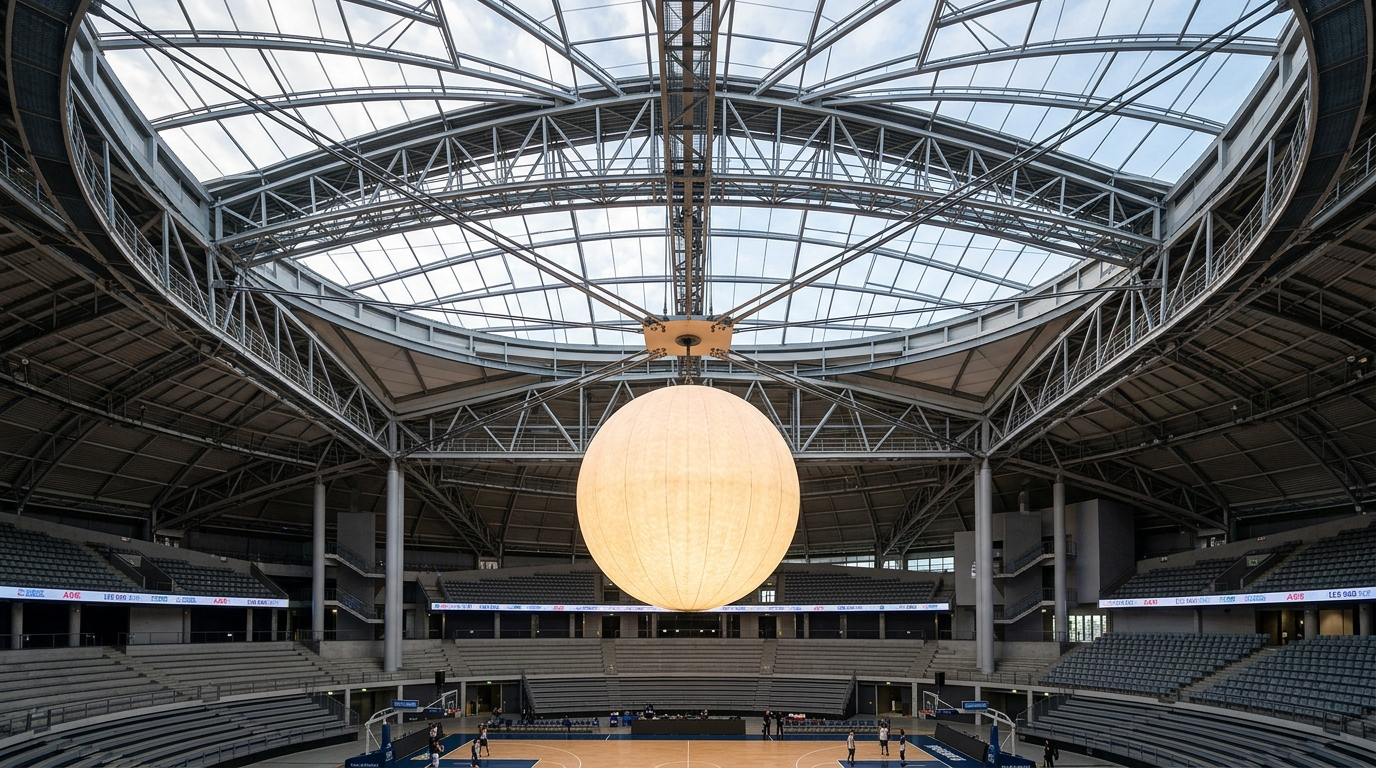
\includegraphics[width=0.48\textwidth]{images/phan2_cau4_dentreo.jpg}\\[2pt]{\footnotesize\itshape Hình minh họa bối cảnh; sử dụng số liệu trong đề.}
\end{center}
\begin{enumerate}[label=\alph*)]
\item Tọa độ của vectơ $\overrightarrow{SA}$ là $(4; 0; 3)$ và độ dài $|\overrightarrow{SA}| = 5\text{ m}$.
\item Cả 4 sợi dây cáp $SA, SB, SC, SD$ có độ dài bằng nhau và bằng $5\text{ m}$.
\item Lực căng trên mỗi sợi dây cáp có độ lớn bằng $\dfrac{2500}{3}\text{ N} \approx 833{,}33\text{ N}$.
\item Góc nghiêng tạo bởi mỗi sợi dây cáp với mặt phẳng nằm ngang $(Oxy)$ bằng $45^\circ$.
\end{enumerate}
\end{minipage}

\end{enumerate}

% ==========================================
% PHẦN III
% ==========================================
\newpage
\section*{PHẦN III. CÂU TRẮC NGHIỆM TRẢ LỜI NGẮN}
\textit{Thí sinh trả lời từ câu 1 đến câu 6. Điền đáp số theo quy chuẩn làm tròn được nêu trong từng câu.}

\begin{enumerate}[label=\textbf{Câu \arabic*:}, leftmargin=*]

\item
\begin{minipage}[t]{\linewidth} 
Một nhà máy hóa chất cần chế tạo một bể chứa hóa chất dạng lăng trụ tam giác đều không nắp có thể tích $V = 16\sqrt{3}\text{ m}^3$. Chi phí làm đáy bể bằng tôn dày là $1{,}2$ triệu đồng/m², chi phí làm các mặt bên bằng tôn mỏng là $0{,}8$ triệu đồng/m². Tìm cạnh đáy $x$ (mét) của lăng trụ để tổng chi phí vật liệu chế tạo bể chứa đạt giá trị nhỏ nhất (làm tròn kết quả đến hàng phần mười, ví dụ điền $5{,}3$).
\begin{center}
    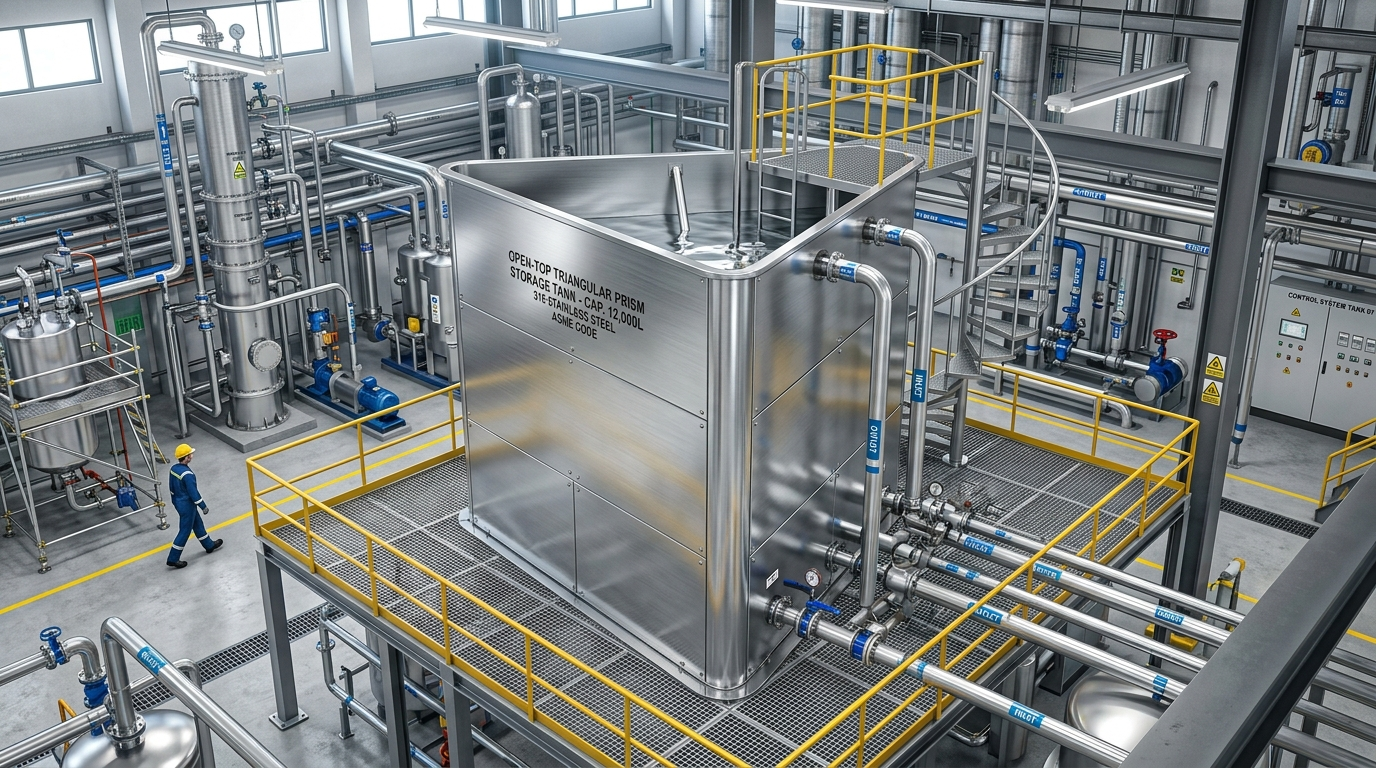
\includegraphics[width=0.48\textwidth]{images/phan3_cau1_bechuahoachat.jpg}\\[2pt]{\footnotesize\itshape Hình minh họa bối cảnh; sử dụng số liệu trong đề.}
\end{center}
\end{minipage}

\item
\begin{minipage}[t]{\linewidth} 
Anh Cường lập kế hoạch tích lũy tài chính mua nhà bằng cách mỗi tháng gửi cố định $15$ triệu đồng vào ngân hàng theo hình thức lãi kép với lãi suất $0{,}6\%$/tháng (tiền gửi vào đầu mỗi tháng). Hỏi sau ít nhất bao nhiêu tháng gửi tiền liên tục thì số dư tài khoản tại cuối tháng đó (sau khi đã cộng lãi tháng) vượt quá $800$ triệu đồng?
\end{minipage}

\item
\begin{minipage}[t]{\linewidth} 
Trong hệ tọa độ $Oxyz$ (đơn vị km, mặt đất là mặt phẳng $z=0$), một trạm ra-đa theo dõi hai thiết bị bay không người lái (UAV) trong khoảng $0 \le t \le 2$ giờ. Hai UAV xuất phát cùng lúc tại thời điểm $t = 0$. UAV thứ nhất bay thẳng đều từ $M(0; 1; 2)$ với vectơ vận tốc $\vec{v}_1 = (2; 1; 1)\text{ (km/h)}$, UAV thứ hai bay thẳng đều từ $N(2; -1; 4)$ với vectơ vận tốc $\vec{v}_2 = (1; 2; -1)\text{ (km/h)}$. Tìm khoảng cách ngắn nhất giữa hai UAV trong quá trình bay (làm tròn kết quả đến hàng phần trăm của km, ví dụ điền $1{,}25$).
\begin{center}
    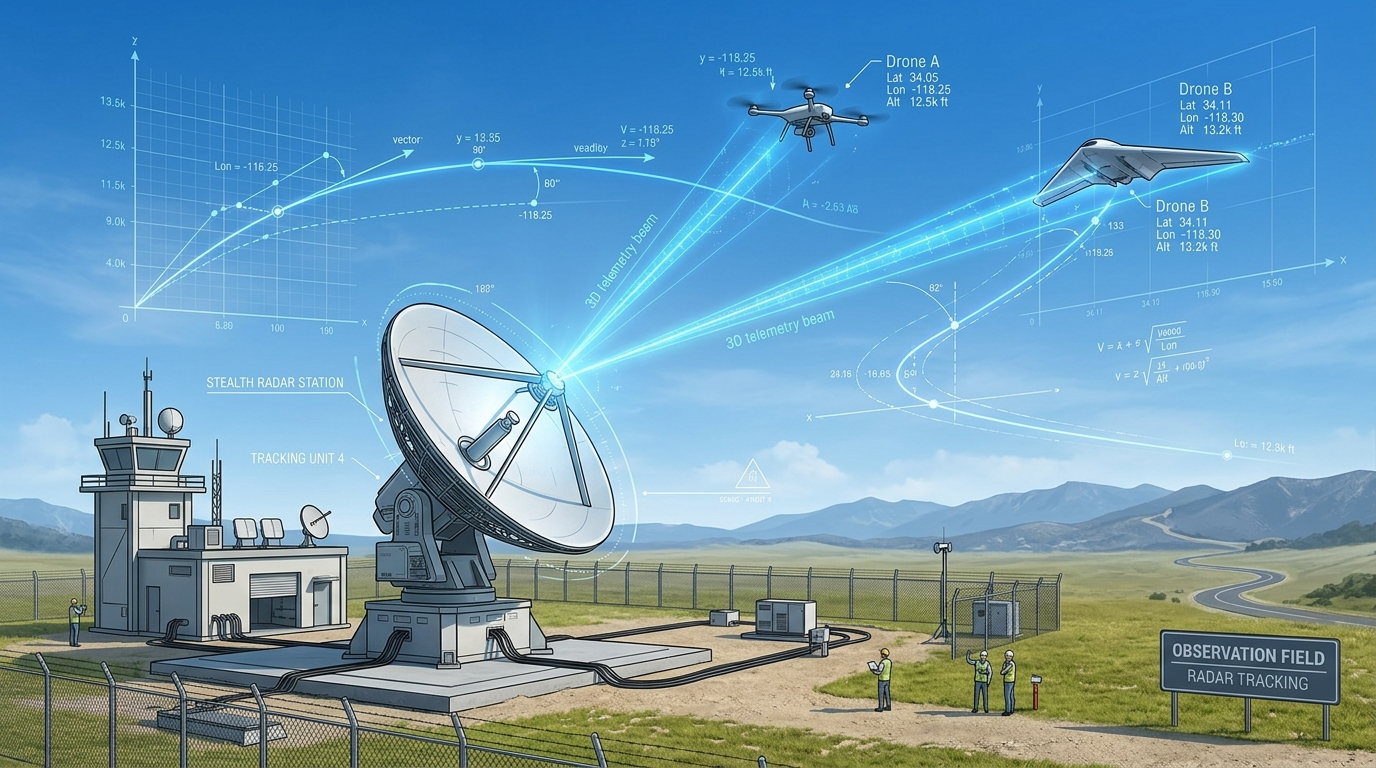
\includegraphics[width=0.48\textwidth]{images/phan3_cau3_rada_uav.jpg}\\[2pt]{\footnotesize\itshape Hình minh họa bối cảnh; sử dụng số liệu trong đề.}
\end{center}
\end{minipage}

\item
\begin{minipage}[t]{\linewidth} 
Một nhà nghiên cứu xã hội khảo sát thu nhập hàng tháng (triệu đồng) của học sinh sau tốt nghiệp thu được bảng tần số ghép nhóm có một số ô bị nhòe mất số liệu ($x, y$ là tần số chưa biết):
\begin{center}
\begin{tabular}{|c|c|c|c|c|c|}
\hline
\textbf{Thu nhập (triệu)} & $[5; 10)$ & $[10; 15)$ & $[15; 20)$ & $[20; 25)$ & $[25; 30)$ \\ \hline
\textbf{Số người} & $10$ & $x$ & $y$ & $12$ & $8$ \\ \hline
\end{tabular}
\end{center}
Biết tổng số người khảo sát là $80$ người và trung vị của mẫu số liệu ghép nhóm bằng $M_e = \dfrac{50}{3}$ triệu đồng. Tìm tần số $y$ của nhóm $[15; 20)$.
\end{minipage}

\item
\begin{minipage}[t]{\linewidth} 
Một ngân hàng thương mại sử dụng thuật toán AI để phân loại rủi ro tín dụng khách hàng vay vốn. Thực tế trong tập hồ sơ có $6\%$ khách hàng thuộc nhóm "rủi ro cao" và $94\%$ thuộc nhóm "rủi ro thấp". Thuật toán AI nhận diện đúng $92\%$ khách hàng rủi ro cao và nhận diện nhầm $5\%$ khách hàng rủi ro thấp (đưa vào danh sách cảnh báo từ chối cho vay). Chọn ngẫu nhiên một khách hàng bị AI đưa vào danh sách cảnh báo, tính xác suất để khách hàng đó thực sự thuộc nhóm "rủi ro cao" (làm tròn kết quả đến chữ số thập phân thứ nhất dưới dạng $\%$, ví dụ điền $54{,}0$).
\end{minipage}

\item
\begin{minipage}[t]{\linewidth} 
Một kỹ sư thiết kế bồn chứa nhiên liệu tên lửa hình tròn xoay thu được khi quay hình phẳng giới hạn bởi đường cong $y = f(x)$, trục hoành $Ox$ và hai đường thẳng $x = 0, x = 4$ xung quanh trục $Ox$. Hàm số $f(x)$ được cho bởi:
$$f(x) = \begin{cases} \sqrt{x+1} & \text{khi } 0 \le x \le 3 \\ \sqrt{7 - x} & \text{khi } 3 < x \le 4 \end{cases}$$
\begin{center}
    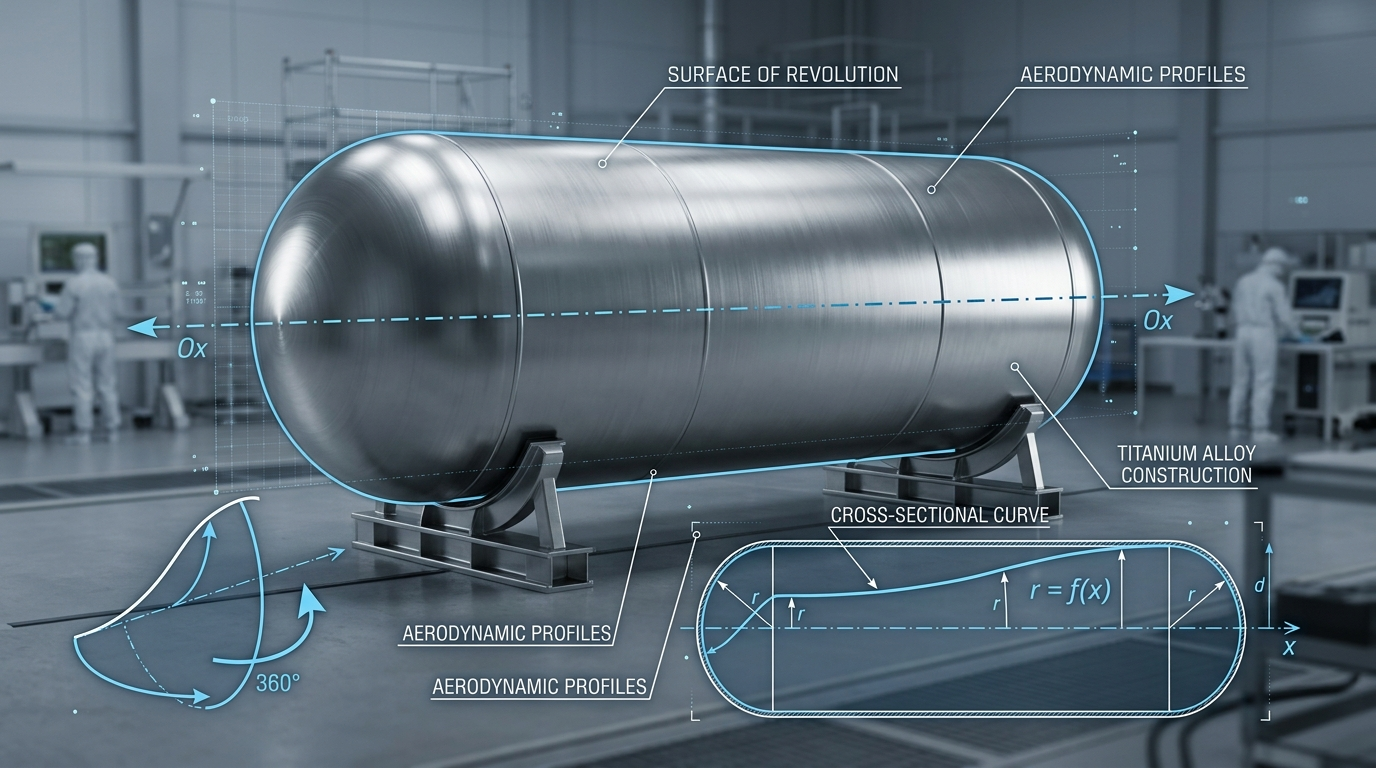
\includegraphics[width=0.48\textwidth]{images/phan3_cau6_bonchuanhienlieu.jpg}\\[2pt]{\footnotesize\itshape Hình minh họa bối cảnh; sử dụng số liệu trong đề.}
\end{center}
Tính thể tích $V$ của bồn chứa nhiên liệu đó (các trục tọa độ có đơn vị mét; viết $V=k\pi\text{ m}^3$ và điền $k$ làm tròn đến hàng phần mười, ví dụ điền $7{,}5$).
\end{minipage}

\end{enumerate}

\newpage
% ==========================================
% BẢNG ĐÁP ÁN TỔNG HỢP
% ==========================================
\section*{BẢNG ĐÁP ÁN TỔNG HỢP}

\subsection*{1. PHẦN I}
\begin{center}
\begin{tabular}{|c|c||c|c||c|c||c|c|}
\hline
\textbf{Câu} & \textbf{Đáp án} & \textbf{Câu} & \textbf{Đáp án} & \textbf{Câu} & \textbf{Đáp án} & \textbf{Câu} & \textbf{Đáp án} \\ \hline
1 & A & 4 & A & 7 & A & 10 & C \\ \hline
2 & B & 5 & B & 8 & D & 11 & C \\ \hline
3 & C & 6 & D & 9 & B & 12 & D \\ \hline
\end{tabular}
\end{center}

\subsection*{2. PHẦN II}
\begin{center}
\begin{tabular}{|c|c|c|c|c|}
\hline
\textbf{Câu} & \textbf{Ý a)} & \textbf{Ý b)} & \textbf{Ý c)} & \textbf{Ý d)} \\ \hline
\textbf{1} & Đúng & Đúng & Sai & Đúng \\ \hline
\textbf{2} & Đúng & Sai & Đúng & Đúng \\ \hline
\textbf{3} & Sai & Đúng & Đúng & Đúng \\ \hline
\textbf{4} & Đúng & Đúng & Đúng & Sai \\ \hline
\end{tabular}
\end{center}

\subsection*{3. PHẦN III}
\begin{center}
\begin{tabular}{|c|c||c|c||c|c|}
\hline
\textbf{Câu} & \textbf{Kết quả điền} & \textbf{Câu} & \textbf{Kết quả điền} & \textbf{Câu} & \textbf{Kết quả điền} \\ \hline
\textbf{1} & 5,3 & \textbf{3} & 1,15 & \textbf{5} & 54,0 \\ \hline
\textbf{2} & 47 & \textbf{4} & 30 & \textbf{6} & 11,0 \\ \hline
\end{tabular}
\end{center}


\newpage
\section*{HƯỚNG DẪN GIẢI CHI TIẾT}
\subsection*{PHẦN I}
\begin{enumerate}[label=\textbf{Câu \arabic*:}, leftmargin=*]
\item \textbf{Đáp án A.} Với $t\ge0$,
\[
C'(t)=\frac{40(4-t^2)}{(t^2+4)^2}.
\]
Hàm tăng trên $[0;2]$ và giảm trên $[2;+\infty)$, nên nồng độ lớn nhất đạt tại $t=2$ giờ.
\item \textbf{Đáp án B.} Sóng âm lan truyền đẳng hướng và không bị hấp thụ nên $I$ tỉ lệ nghịch với bình phương khoảng cách. Do đó $I_B/I_A=(10/100)^2=1/100$ và $L_B=90+10\log_{10}(1/100)=70$ dB.
\item \textbf{Đáp án C.}
\[
W=\int_{0{,}1}^{0{,}3}(200x+60x^2)\,dx
 =[100x^2+20x^3]_{0{,}1}^{0{,}3}=8{,}52\text{ J}.
\]
\item \textbf{Đáp án A.} Mặt phẳng có pháp tuyến $\vec n=(2;-2;1)$ và $\|\vec n\|^2=9$. Tại $A(1;2;3)$, $2x-2y+z+8=9$. Hình chiếu là
\[
M=A-\frac{9}{9}\vec n=(-1;4;2).
\]
Thay tọa độ này vào phương trình mặt phẳng cho giá trị $0$.
\item \textbf{Đáp án B.} Gọi $u_0=0$, khi đó $u_n=0{,}4u_{n-1}+100$ và
\[
u_n=100\frac{1-0{,}4^n}{1-0{,}4}\longrightarrow\frac{500}{3}\approx166{,}67\text{ mg}.
\]
\item \textbf{Đáp án D.} Giá trị đại diện các nhóm là $19,21,23,25$.
\[
\bar x=\frac{10\cdot19+25\cdot21+10\cdot23+5\cdot25}{50}=21{,}4.
\]
\[
s^2=\frac{10(19-21{,}4)^2+25(21-21{,}4)^2+10(23-21{,}4)^2+5(25-21{,}4)^2}{50}=3{,}04.
\]
Vì thế $s=\sqrt{3{,}04}\approx1{,}74$ mm.
\item \textbf{Đáp án A.} Dùng biến cố đối và tính độc lập: $P=1-(1-0{,}02)^{10}=1-0{,}98^{10}\approx18{,}29\%$.
\item \textbf{Đáp án D.} Gọi $D$ là biến cố có bệnh và $+$ là kết quả dương tính. Theo công thức Bayes,
\[
P(D\mid +)=\frac{0{,}01\cdot0{,}96}{0{,}01\cdot0{,}96+0{,}99\cdot0{,}05}
 =\frac{32}{197}\approx16{,}24\%.
\]
\item \textbf{Đáp án B.} Ta có $y=x-2+1/(x-1)$, $x\ne1$, và $y'=1-1/(x-1)^2$. Đạo hàm đổi dấu tại $x=0,2$; hai điểm cực trị là $(0;-3)$ và $(2;1)$. Khoảng cách bằng $\sqrt{2^2+4^2}=2\sqrt5$.
\item \textbf{Đáp án C.} $P'(t)=-3t^2+18t+48=-3(t-8)(t+2)$. Trên $[0;10]$, hàm tăng đến $t=8$ rồi giảm, nên đạt công suất lớn nhất lúc $6+8=14$ giờ.
\item \textbf{Đáp án C.} Đặt $X=A+\lambda(B-A)$ với $0\le\lambda\le1$. Khi đó
\[
OX^2=(2+6\lambda)^2+(1+8\lambda)^2+10^2
 =105+40\lambda+100\lambda^2.
\]
Biểu thức tăng trên $[0;1]$, nên khoảng cách nhỏ nhất đạt tại $A$ và bằng $\sqrt{105}$ km. Hình chiếu lên đường thẳng $AB$ ứng với $\lambda=-1/5$ nằm ngoài đoạn bay, nên kết quả $\sqrt{101}$ không phù hợp với đề.
\item \textbf{Đáp án D.} Dùng phương pháp đĩa tròn:
\[
V=\pi\int_0^2(\sqrt{x}e^{x/2})^2\,dx
 =\pi\int_0^2xe^x\,dx=\pi[(x-1)e^x]_0^2=\pi(e^2+1)\text{ dm}^3.
\]
\end{enumerate}

\subsection*{PHẦN II}
\begin{enumerate}[label=\textbf{Câu \arabic*:}, leftmargin=*]
\item \textbf{a) Đúng; b) Đúng; c) Sai; d) Đúng.}
\begin{itemize}[leftmargin=*]
\item a) $R(x)=x(150-6x)=150x-6x^2$.
\item b) $C'(x)=6x^2-24x+30$, nên $C'(3)=12$ triệu đồng/ngàn thiết bị.
\item c) Khi bỏ thuế, $L_0(x)=-2x^3+6x^2+120x-40$, tăng đến $x=1+\sqrt{21}\approx5{,}58$ rồi giảm. Với sản lượng nguyên, chỉ cần so sánh $L_0(5)=460$ và $L_0(6)=464$. Lợi nhuận tối đa là $464$ triệu đồng tại $x=6$, tăng $464-370=94$ triệu đồng, không phải $120$ triệu đồng.
\item d) Khi có thuế, $L(x)=-2x^3+6x^2+102x-40$ và $L'(x)=-6(x^2-2x-17)$. Điểm tối ưu liên tục là $1+3\sqrt2\approx5{,}24$. Với $x$ nguyên, so sánh $L(5)=370$ và $L(6)=356$, suy ra tối ưu tại $x=5$. Không được đồng nhất tối ưu nguyên với tối ưu liên tục.
\end{itemize}
\item \textbf{a) Đúng; b) Sai; c) Đúng; d) Đúng.}
Từ $v(0)=0$ và $h(0)=0$, trong $0\le t\le4$:
\[
v(t)=6t^2-t^3,\qquad h(t)=2t^3-\frac{t^4}{4}.
\]
\begin{itemize}[leftmargin=*]
\item a) $v(4)=96-64=32$ m/s.
\item b) Sau khi hết nhiên liệu, độ cao tăng thêm $32^2/(2\cdot10)=51{,}2$ m. Tổng độ cao tối đa bằng $64+51{,}2=115{,}2$ m, nên mệnh đề $83{,}2$ m sai.
\item c) $h(4)=128-64=64$ m.
\item d) Tên lửa bay lên thêm trong $\Delta t=32/10=3{,}2$ s.
\end{itemize}
\item \textbf{a) Sai; b) Đúng; c) Đúng; d) Đúng.}
Gọi $C$ là biến cố tin nhắn bị chặn sau hai lớp. Tỉ lệ phát hiện ở lớp 2 trong đề đã được cho trên tập tin nhắn được AI chuyển đến.
\begin{itemize}[leftmargin=*]
\item a) Với tin nhắn hợp lệ, lớp 2 không bao giờ chặn nhầm, nên $P(C\mid\overline A)=0$, không phải $3{,}68\%$.
\item b) $P(B)=0{,}08\cdot0{,}95+0{,}92\cdot0{,}04=0{,}1128$.
\item c) $P(A\mid B)=0{,}076/0{,}1128\approx67{,}38\%$.
\item d) Xác suất đồng thời là tin nhắn rác và bị chặn là $P(A\cap C)=0{,}08\cdot0{,}95\cdot0{,}98=0{,}07448$. Cần phân biệt với $P(C\mid A)=0{,}95\cdot0{,}98=0{,}931$.
\end{itemize}
\item \textbf{a) Đúng; b) Đúng; c) Đúng; d) Sai.}
\begin{itemize}[leftmargin=*]
\item a), b) Các vectơ từ $S$ đến điểm treo là $(4;0;3)$, $(0;4;3)$, $(-4;0;3)$, $(0;-4;3)$; tất cả có độ dài $\sqrt{16+9}=5$ m.
\item c) Theo giả thiết lực căng bằng nhau, các thành phần ngang triệt tiêu. Thành phần thẳng đứng mỗi dây là $3T/5$, nên $4\cdot3T/5=2000$, suy ra $T=2500/3\approx833{,}33$ N.
\item d) Góc $\theta$ với mặt phẳng ngang thỏa mãn $\sin\theta=3/5$, nên $\theta\approx36{,}87^\circ$, không phải $45^\circ$.
\end{itemize}
\end{enumerate}

\subsection*{PHẦN III}
\begin{enumerate}[label=\textbf{Câu \arabic*:}, leftmargin=*]
\item \textbf{Kết quả điền: $5{,}3$.} Gọi $h$ là chiều cao bể, $x>0$ là cạnh tam giác đều ở đáy. Từ thể tích:
\[
\frac{\sqrt3}{4}x^2h=16\sqrt3\quad\Longrightarrow\quad h=\frac{64}{x^2}.
\]
Bể không nắp có một đáy và ba mặt bên, nên chi phí (triệu đồng) là
\[
C(x)=1{,}2\frac{\sqrt3}{4}x^2+0{,}8\cdot3xh
 =0{,}3\sqrt3\,x^2+\frac{153{,}6}{x}.
\]
$C'(x)=0{,}6\sqrt3\,x-153{,}6/x^2=0$ cho $x=\sqrt[3]{256/\sqrt3}\approx5{,}2872$. Do $C''(x)=0{,}6\sqrt3+307{,}2/x^3>0$, đây là cực tiểu duy nhất và cũng là giá trị nhỏ nhất trên $x>0$. Làm tròn đến hàng phần mười được $5{,}3$ m.
\item \textbf{Kết quả điền: $47$.} Mỗi khoản gửi đầu tháng được hưởng lãi của chính tháng đó. Số dư cuối tháng thứ $n$ (triệu đồng) là
\[
S_n=15\sum_{j=1}^n1{,}006^j
 =15\cdot1{,}006\frac{1{,}006^n-1}{0{,}006}.
\]
Dãy tăng và $S_{46}\approx796{,}655<800$, $S_{47}\approx816{,}525>800$, nên cần ít nhất $47$ tháng.
\item \textbf{Kết quả điền: $1{,}15$.} Vị trí hai UAV tại thời điểm $t$ là
\[
M_t=(2t;1+t;2+t),\qquad N_t=(2+t;-1+2t;4-t).
\]
Với $0\le t\le2$, hai UAV đều ở phía trên mặt đất. Bình phương khoảng cách:
\[
d^2(t)=(t-2)^2+(2-t)^2+(2t-2)^2
 =6t^2-16t+12=6\left(t-\frac43\right)^2+\frac43.
\]
Do $4/3\in[0;2]$, khoảng cách nhỏ nhất là $\sqrt{4/3}=2/\sqrt3\approx1{,}1547$ km, làm tròn được $1{,}15$.
\item \textbf{Kết quả điền: $30$.} Tổng tần số cho $x+y=50$. Trung vị thuộc nhóm $[15;20)$, nên
\[
\frac{50}{3}=15+\frac{40-(10+x)}{y}\cdot5
 \quad\Longrightarrow\quad 30-x=\frac y3.
\]
Kết hợp với $x+y=50$ suy ra $x=20$, $y=30$. Kiểm tra: tần số tích lũy trước nhóm là $30<40$ và sau nhóm là $60>40$, đúng nhóm chứa trung vị.
\item \textbf{Kết quả điền: $54{,}0$.} Theo công thức Bayes:
\[
P(\text{rủi ro cao}\mid\text{cảnh báo})
 =\frac{0{,}06\cdot0{,}92}{0{,}06\cdot0{,}92+0{,}94\cdot0{,}05}
 =\frac{276}{511}\approx54{,}01174168\%.
\]
Làm tròn trực tiếp kết quả cuối cùng đến một chữ số thập phân được $54{,}0\%$.
\item \textbf{Kết quả điền: $11{,}0$.} Tiết diện vuông góc với trục quay là đĩa tròn bán kính $f(x)$, nên
\[
V=\pi\left[\int_0^3(x+1)\,dx+\int_3^4(7-x)\,dx\right]
 =\pi\left(\frac{15}{2}+\frac72\right)=11\pi\text{ m}^3.
\]
Vì $V=k\pi\text{ m}^3$, ta điền hệ số $k=11{,}0$, không điền giá trị $11\pi$ hay $34{,}6$.
\end{enumerate}

\end{document}
